\documentclass{article}

%
% Hyphenation etc...
%
\usepackage{polyglossia}
\setdefaultlanguage[variant=british]{english}
\usepackage{csquotes}

%
% General document formatting
%
\usepackage{url}
\usepackage{xcolor}
% \usepackage[margin=0.7in]{geometry}
% \usepackage[parfill]{parskip}
% \usepackage[utf8]{inputenc}  % Not needed under xelatex

%
% Related to math
%
\usepackage{amsmath,amssymb,amsfonts,amsthm}

%
% Change tracking
%
\usepackage{changes}
\definechangesauthor[name={John Reid}, color=orange]{JR}

%
% Bibliography
%
\usepackage[
    backend=biber,
    % doi=false,
    isbn=false,
    url=false,
    % style=apa,
    % style=humanmutation,
    sorting=none,
    natbib=true,
  ]{biblatex}
\bibliography{CAGI5-reg-sat} % or
% \addbibresource{<database>.<extension>}


%
% Command definitions
%
\newcommand{\todo}[1]{\textcolor{red}{TODO: #1}}


\begin{document}

We were inspired by Zeng et al.'s winning
method~\cite{ZengAccurateeQTLprioritization2017} from the CAGI~4
challenge~\citep{KreimerPredictinggeneexpression2017}.

All code to reproduce the submitted results is available in a git
repository~\url{git@bitbucket.org:alex-hh/cagimpra.git} which can be made
available on request.


\section*{Introduction}

\subsection*{Biological context}


\subsection*{Existing/similar methods}

\subsection*{Data}

\todo{Describe training and test data.}

\begin{figure}
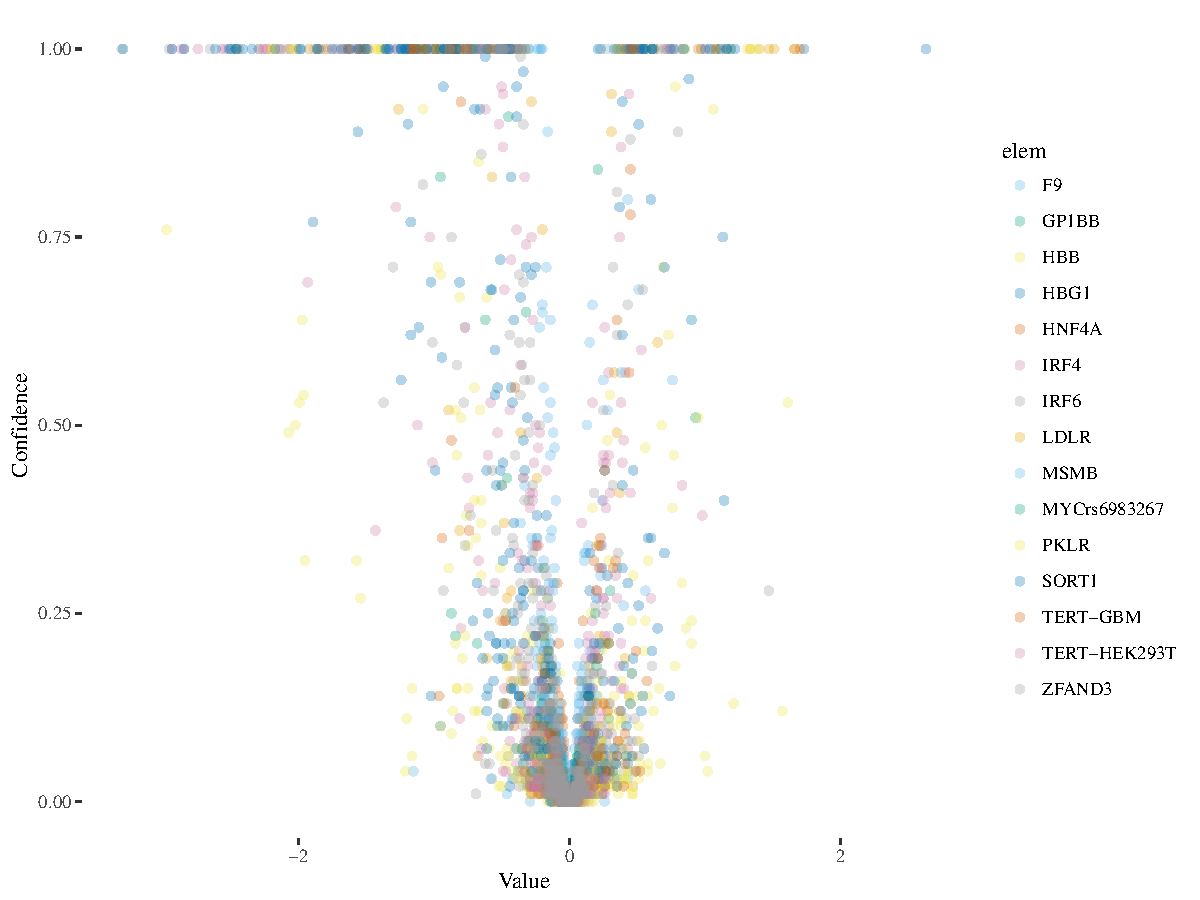
\includegraphics[width=\textwidth]{fig-conf-value-scatter}
\caption{Scatter plot of the confidence and value scores in the training data coloured
by regulatory element and cell line.}
\label{fig:conf-value}
\end{figure}

\begin{figure}
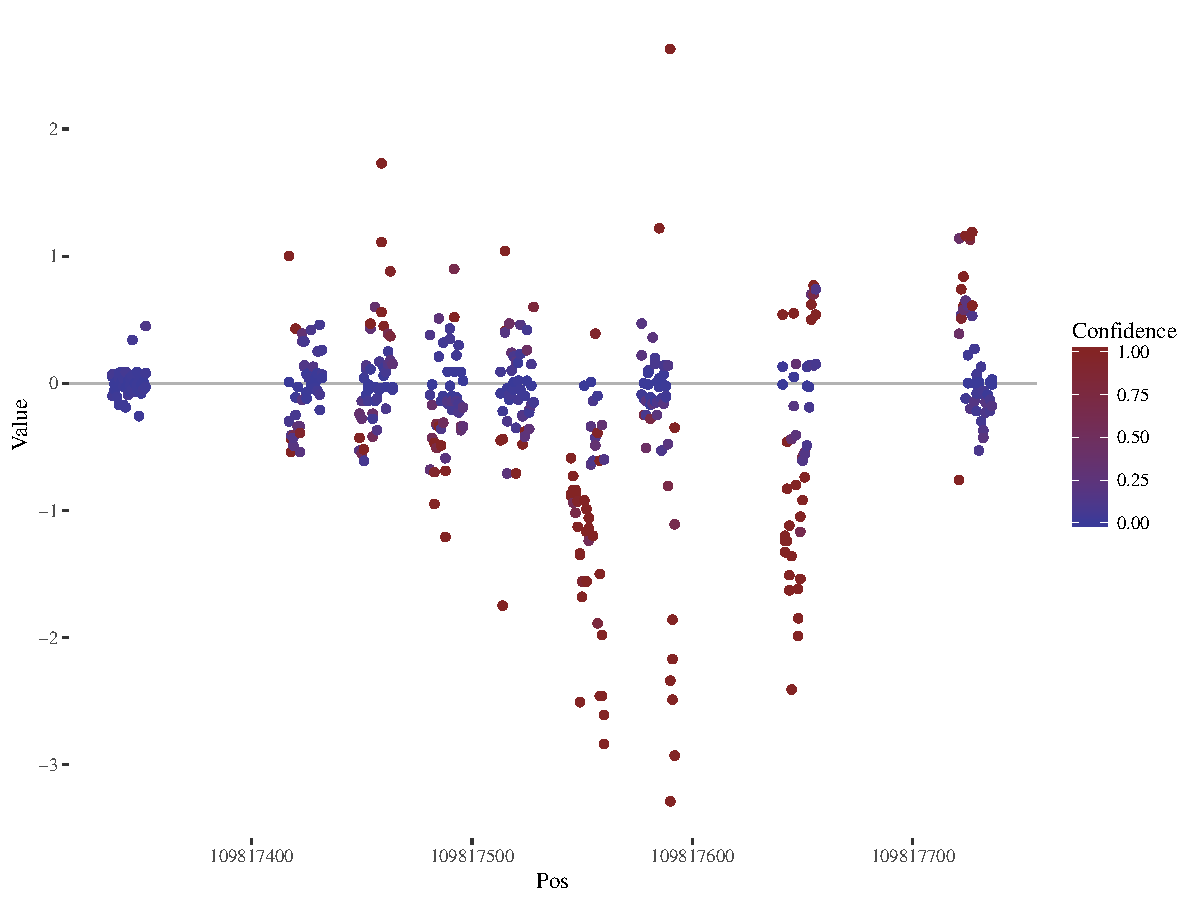
\includegraphics[width=\textwidth]{fig-value-conf-SORT1}
\caption{Training data for the SORT1 regulatory element.}
\label{fig:training-sort1}
\end{figure}



\section*{Methods}


\subsection*{Features}

We tested different types of feature to assess their predictive power.


\subsubsection*{Conservation}

We used \emph{phyloP}~\cite{PollardDetectionnonneutralsubstitution2010},
\emph{phastCons}~\cite{SiepelEvolutionarilyconservedelements2005}, \emph{GerpN}
and \emph{GerpRS}~\cite{CooperDistributionintensityconstraint2005a} base-pair
resolved conservation scores.

Downloaded from UCSC~\cite{KuhnUCSCgenomebrowser2013}?


\subsubsection*{DNase hypersensitivity}

For each regulatory element we identified the closest matching
ENCODE~\cite{DunhamintegratedencyclopediaDNA2012} cell type for which there is
a DNase-hypersensitivity track (see Table~\ref{tab:encode-cell-types}). We
downloaded the tracks~\cite{RosenbloomENCODEDataUCSC2012} and created
41-dimensional features consisting of the signal at each base-pair flanked by
the signal at the bases 20bp on either side.

\begin{table}[htp]
\resizebox{\textwidth}{!} {
\begin{tabular}{rll}
  \\
  challenge  & ENCODE    & UCSC track \\
  \hline
  HepG2      & HepG2     & wgEncodeOpenChromDnaseHepg2BaseOverlapSignal \\
  HEL 92.1.7 & GM12878   & wgEncodeOpenChromDnaseGm12878BaseOverlapSignal \\
  HEK293T    & HEK293T   & wgEncodeOpenChromDnaseHek293tBaseOverlapSignal \\
  K562       & K562      & wgEncodeOpenChromDnaseK562BaseOverlapSignalV2 \\
  GBM        & Gliobla   & wgEncodeOpenChromDnaseGlioblaBaseOverlapSignal \\
  SK-MEL-28  & Colo829   & wgEncodeOpenChromDnaseColo829BaseOverlapSignal \\
  HaCaT      & NHEK      & wgEncodeOpenChromDnaseNhekBaseOverlapSignal \\
  MIN6       & PanIslets & wgEncodeOpenChromDnasePanisletsBaseOverlapSignal
\end{tabular}
}
\caption{The ENCODE cell lines that were identified as the closest
matches to the cell lines in the challenge. The corresponding UCSC track
names are also given.}
\label{tab:encode-cell-types}
\end{table}


\subsubsection*{DeepSea neural networks}

We trained several different neural network architectures on the genomic
prediction benchmark detailed in the original DeepSea
paper~\cite{ZhouPredictingeffectsnoncoding2015}. We evaluated these networks on
a region surrounding each variant twice, once with the reference allele and
once with the alternate allele. Features were generated as the difference in
activations between the two evaluations of internal and output layers of the
networks.

DanQ network~\cite{QuangDanQhybridconvolutional2016}.


\subsubsection*{Region identity}

We one-hot encoded the identity of region to use as a feature.


\subsubsection*{Substitution}

We one-hot encoded the reference to alternate allele substitution as a feature.


\subsubsection*{Stacked predictions}

We generated features representing the \texttt{Value} and \texttt{Confidence}
by fitting models to held out data. For the submissions, the held out data was
the training data. For the cross-validation, the held out data was the training
folds. We used the DeepSea difference features, DNase features and conservation
features to fit the models.

\begin{figure}
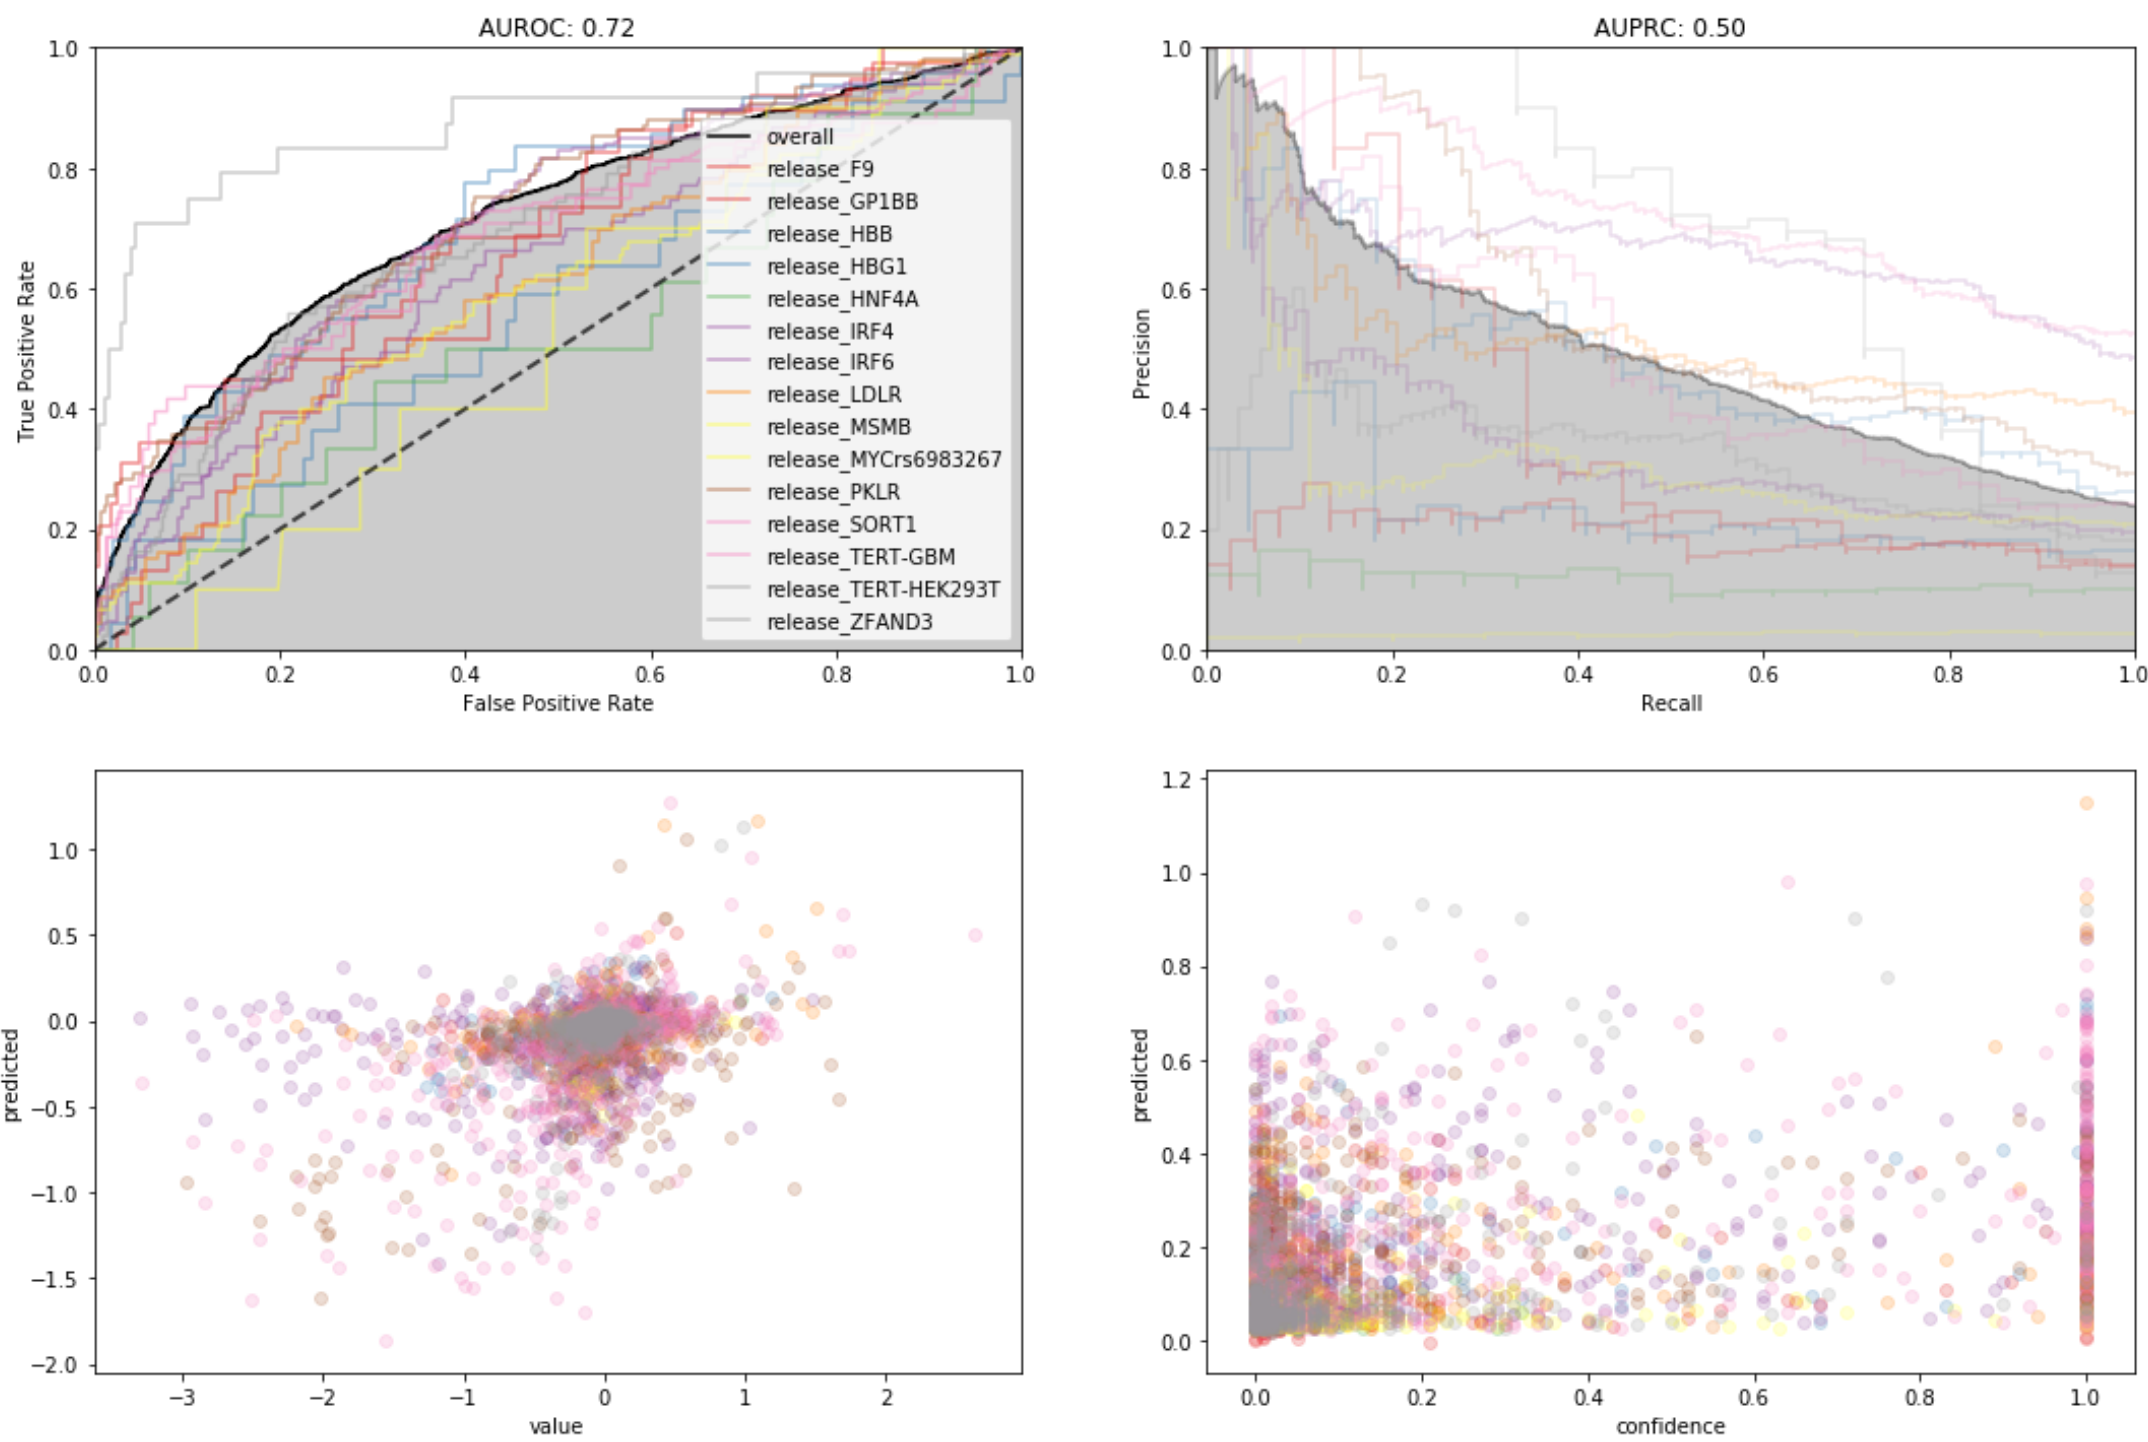
\includegraphics[width=\textwidth]{fig-stacking-x-validation}
\caption{Predictions used for stacking coloured by regulatory element.
  \emph{Top left}: Overall and regulatory element specific AUROC for prediction
  of \texttt{Direction} using \texttt{Value}.
  \emph{Top right}: Overall and regulatory element specific AUPRC for prediction
  of \texttt{Direction} using \texttt{Value}.
  \emph{Bottom left}: Predicted \texttt{Value} against actual \texttt{Value}.
  \emph{Bottom right}: Predicted \texttt{Confidence} against actual \texttt{Confidence}.
}
\label{fig:stacking}
\end{figure}


\subsection*{Inference}


\subsubsection*{Models}

We used three different gradient boosting algorithms:
\emph{XGBoost}~\cite{ChenXGBoostScalableTree2016},
\emph{CatBoost}~\cite{ProkhorenkovaCatBoostunbiasedboosting2017} and
\emph{LightGBM}~\cite{KeLightGBMHighlyEfficient2017}. We used the gradient
boosting algorithms to regress the \texttt{Value} and \texttt{Confidence}, we
also used them as classifers to predict the \texttt{Direction}. We tested
different subsets of features in a 5-fold cross-validation set up to identify
the best features.  Models were assessed by the cross-validated one against
many area-under-precision-recall-curve (AUPRC). We stacked models in that we
used the prediction of cross-validated regression models of the \texttt{Value}
and \texttt{Confidence} as features in the classification model for the
\texttt{Direction}.

\subsubsection*{Cross-validation}

\todo{Describe cross-validation scheme respecting structure of training loci}



\subsubsection*{Hyper-parameter Bayesian optimisation}

\todo{Describe Bayesian optimisation scheme}


\subsubsection*{Confidence standard error}

To estimate the standard error of the \texttt{Confidence} we trained an
ensemble of regression models and used the standard deviation of the
predictions to estimate the standard error.


\subsection*{Variable importance}

\todo{Discuss which features were important for prediction.}


\section*{Contributions}

HK, AHH and JR developed the deep convolutional neural network models of
genomic sequence. AHH and JR derived the features required for this
project. AHH and JR fit the gradient boosting machines. JR wrote the
manuscript.


\subsection*{Acknowledgements}

We would like to thank Elena Vigorito, Lorenz Wernisch, Paul Newcombe, and Paul
Kirk for insightful comments on parts of this work.

%
% Bibliography
%
\printbibliography

\end{document}
